\section{Цель работы}
Освоение принципов построения адаптивной системы управления многомерным объектом.


\section{Теоретические сведения}
Рассматриваемый объект управления:
\begin{equation}
    \begin{aligned}
        & \dot{x} = Ax + bu, \\
        & y = Cx,
    \end{aligned}
\end{equation}
где $x \in \mathbb{R}^n$~--- вектор состояния, $y, u \in \mathbb{R}^1$~--- регулируемая переменная и сигнал управления соответственно, 
\begin{equation}
    A =
    \begin{bmatrix}
        0 & 1 & 0 & \ldots & 0 \\
        0 & 0 & 1 & \ldots & 0 \\
        \vdots & \vdots & \vdots & \ddots & \vdots \\
        0 & 0 & 0 & \ldots & 1 \\
        -a_0 & -a_1 & -a_2 & \ldots & -a_{n-1}
    \end{bmatrix}\!\!,
    \qquad
    b =
    \begin{bmatrix}
        0 \\ 0 \\ \vdots \\ 0 \\ b_0
    \end{bmatrix}\!\!,
    \qquad
    C =
    \begin{bmatrix}
        1 & 0 & \ldots & 0 & 0
    \end{bmatrix}\!\!,
\end{equation}
$a_i, i=\overline{0, n-1}$~--- неизвестные параметры, $b_0$~--- известный параметр.

Задача управления заключается в компенсации параметрической неопределенности объекта и обеспечении следующего целевого равенства:
\begin{equation}\label{eq_goal_of_control}
    \lim_{t \rightarrow \infty} \bigl( x_m(t) - x(t) \bigr) = \lim_{t \rightarrow \infty} e(t) = 0,
\end{equation}
где $e = x_m - x$~--- вектор ошибки управления, $x_m \in \mathbb{R}^n$~--- вектор, генерируемый эталонной моделью
\begin{equation}
    \begin{aligned}
        & \dot{x}_M = A_M x_M + b_M g, \\
        & y_M = C_M x_M,
    \end{aligned}
\end{equation}
с задающим воздействием $g(t)$ и матрицами вида
\begin{equation}
    A_M =
    \begin{bmatrix}
        0 & 1 & 0 & \ldots & 0 \\
        0 & 0 & 1 & \ldots & 0 \\
        \vdots & \vdots & \vdots & \ddots & \vdots \\
        0 & 0 & 0 & \ldots & 1 \\
        -a_{M0} & -a_{M1} & -a_{M2} & \ldots & -a_{Mn-1}
    \end{bmatrix}\!\!,
    \qquad
    b_M =
    \begin{bmatrix}
        0 \\ 0 \\ \vdots \\ 0 \\ a_{M0}
    \end{bmatrix}\!\!,
    \qquad
    C_M =
    \begin{bmatrix}
        1 & 0 & \ldots & 0 & 0
    \end{bmatrix}\!\!,
\end{equation}

Решающие поставленную задачу настраиваемый регулятор
\begin{equation}\label{eq_tuned_controller}
    u = \frac{1}{b_0} (\hat\theta^T x + a_{M0} g),
\end{equation}
и алгоритм адаптации
\begin{equation}\label{eq_AA}
    \dot{\hat{\theta}} = \gamma x k^T P e \ldotp
\end{equation}
где $k = [0\;\ldots\;0\;1]^T$, $P=P^T \succ 0$~--- матрица, являющаяся решением уравнения $A^T_M P + P A_M =$\\ $=-Q$, где $\forall Q : Q=Q^T \succ 0$


\section{Исходные данные}
Варианту \textnumero2 соответствует следующий набор исходных данных:
\begin{equation}
    A =
    \begin{bmatrix}
        0 & 1 \\
        1 & -1
    \end{bmatrix}\!\!,
    \qquad
    b_0 = 2,
    \qquad
    t_\text{п} = 0.3 \text{ с},
    \qquad
    \sigma = 0\%,
    \qquad
    g(t) = \cos t + 3\sin 2t + 5 \ldotp
\end{equation}


\section{Результаты расчетов и моделирования}
\subsection{Построение эталонной модели}
Для обеспечения требуемых показателей качества в качестве характеристического полинома матрицы $A_M$ выбран стандартный полином Ньютона второго порядка
\begin{equation}
    (\lambda + \omega_0)^2 = \lambda^2 + 32 \lambda + 256
\end{equation}
где
\begin{equation}
    \omega_0 = \frac{4.8}{t_\text{п}} = \frac{4.8}{0.3} = 16
\end{equation}
где, в свою очередь, $4.8$~с~--- стандартное время переходного процесса.
Итого матрица~$A_M$ имеет следующий вид
\begin{equation}
    A_M =
    \begin{bmatrix}
        0 & 1\\ 
        -256 & -32
    \end{bmatrix} \!\!\ldotp
\end{equation}

График переходной функции эталонной модели и ее схема моделирования показаны на рисунке~\ref{img_ref_model}.

\begin{figure}[h]
	\begin{minipage}[h]{0.36\linewidth}
		\center{ 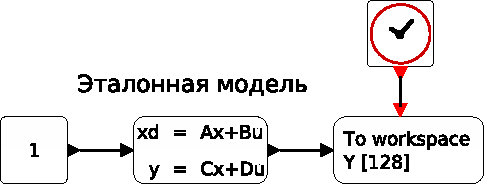
\includegraphics[height = 2.7 cm]{ref_model_scheme.pdf} }
	\end{minipage}
	\hfill
	\begin{minipage}[h]{0.59\linewidth}
		\centering{ 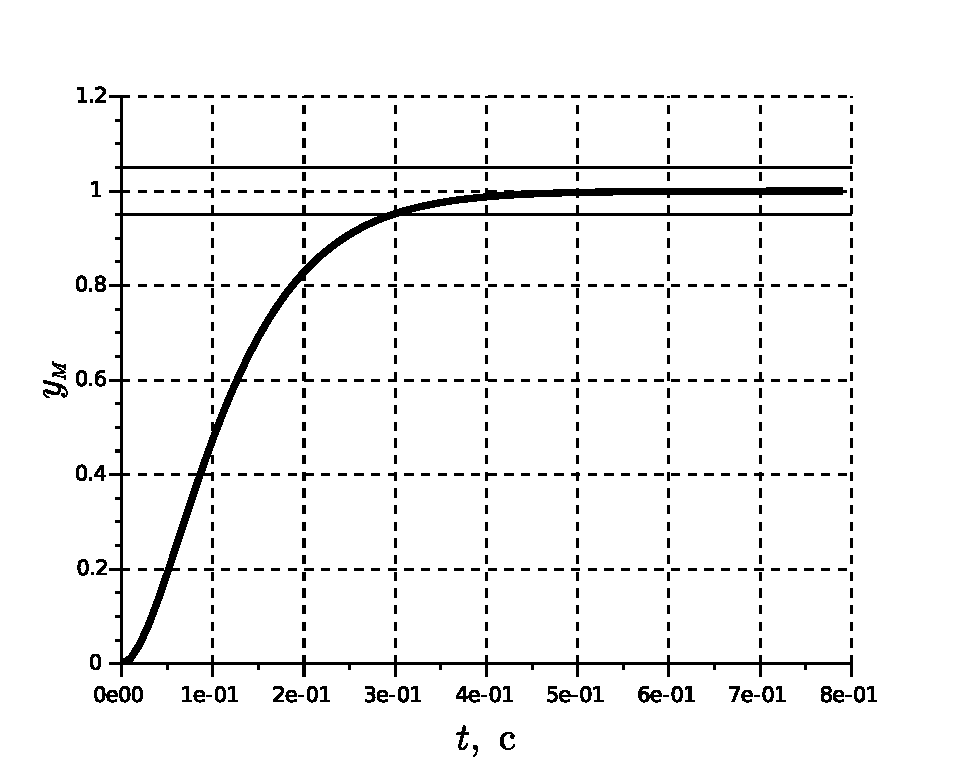
\includegraphics[height = 8.5 cm]{ref_model_trans_func.pdf} }
	\end{minipage}
	\caption{Схема моделирования и график переходной функции эталонной модели.}
	\label{img_ref_model}
\end{figure}

\subsection{Моделирование работы неадаптивной системы}
Результаты моделирования неадаптивной системы управления и соответствующая схема моделирования показаны на рисунках~\ref{img_no_adapt}--\ref{img_no_adapt_unstable}.

\begin{figure}[h!]
    \centering
    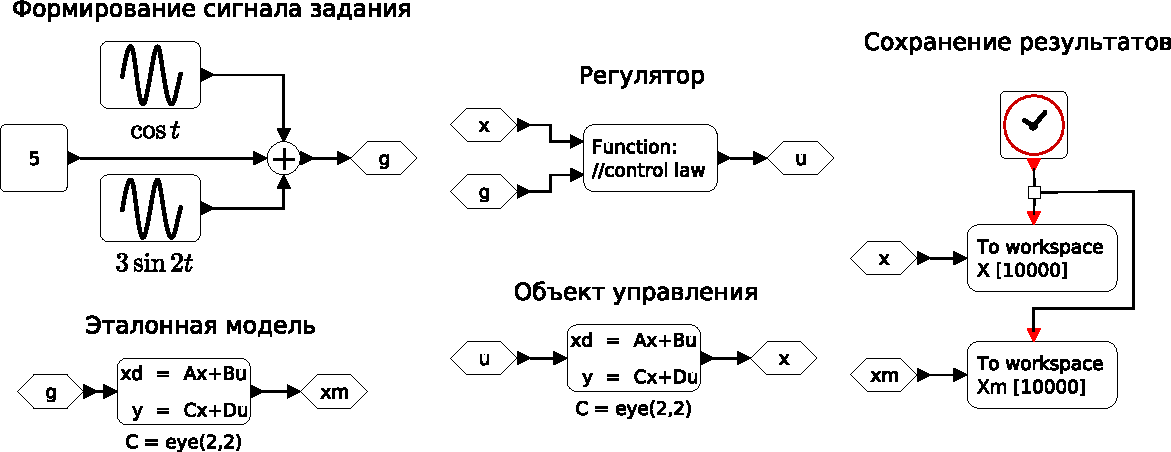
\includegraphics[width=0.9\textwidth]{no_adapt.pdf}
    \vspace{0.4cm}
    \caption{Схема моделирования процесса работы рассматриваемой системы под управлением ненастраиваемого регулятора.}
    \label{img_no_adapt}
\end{figure}

\begin{figure}[h!]
    \centering
    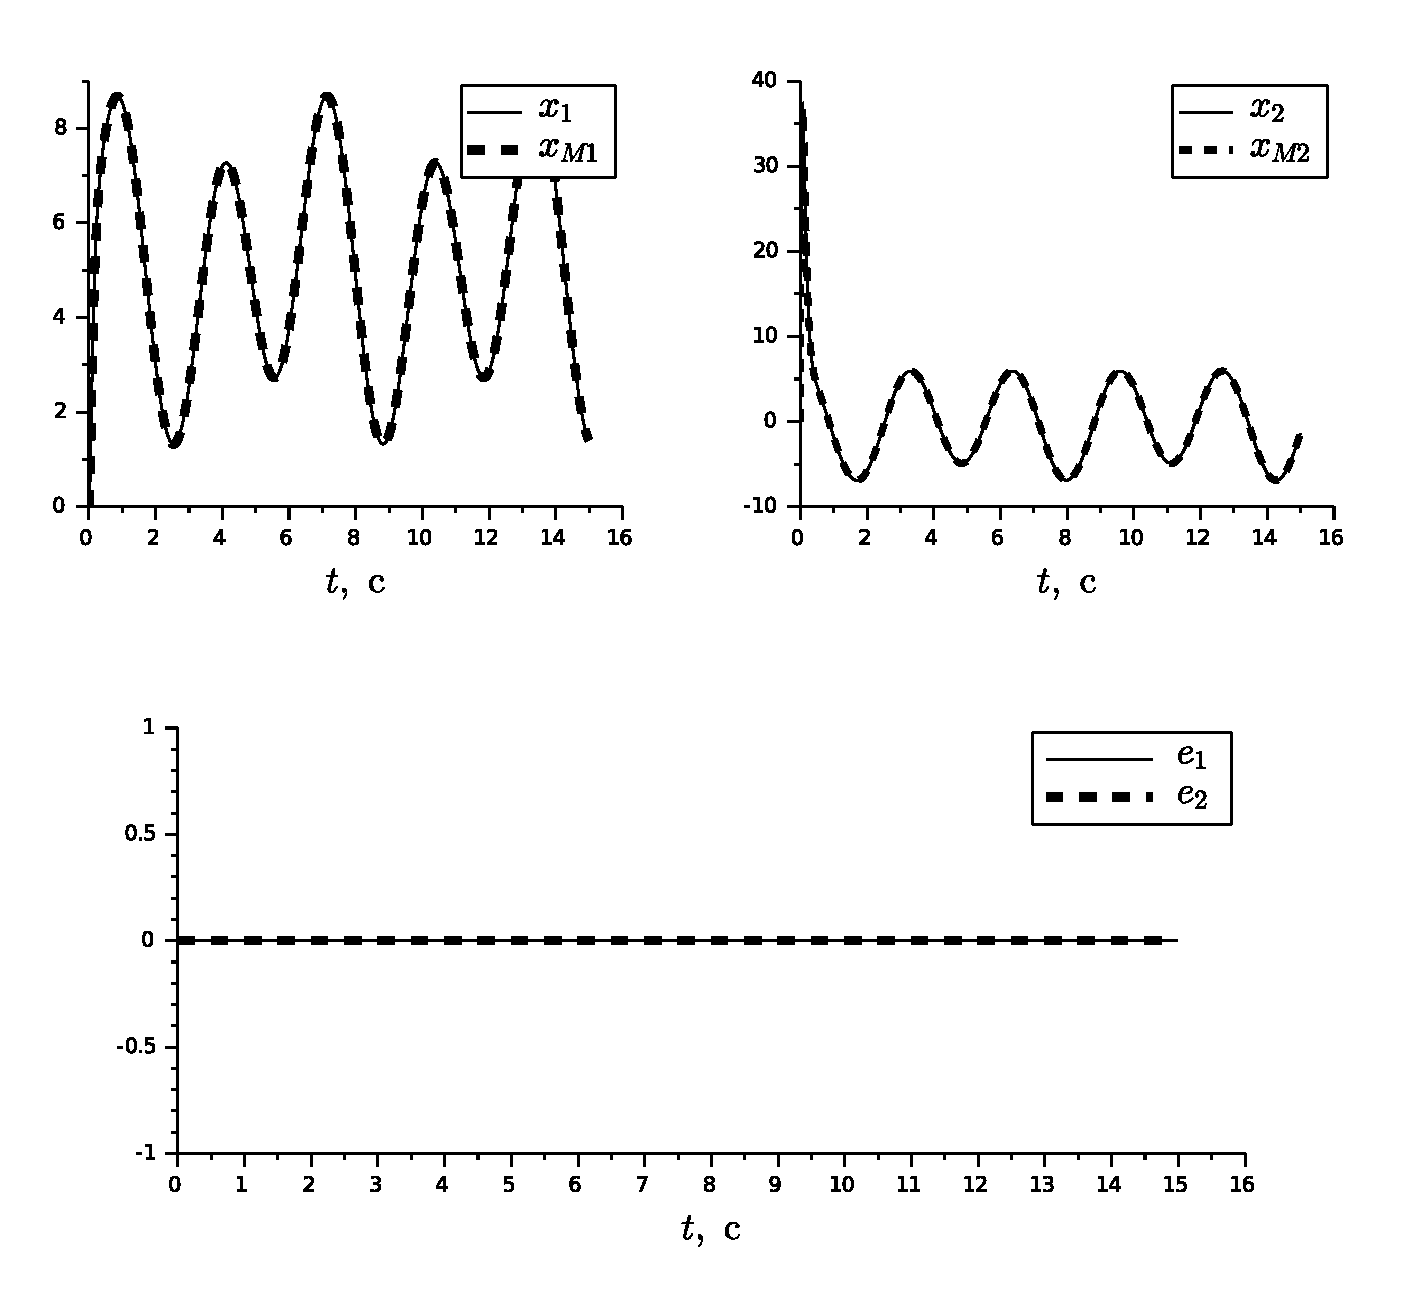
\includegraphics[width=0.79\textwidth]{no_adapt_nominal.pdf}
    \caption{Графики переходных процессов при $a_0=-1$, $a_1 = 1$ ($\theta_1 = -257$, $\theta_2 = -31$).}.
    \label{img_no_adapt_nominal}
\end{figure}

\begin{figure}[h!]
    \centering
    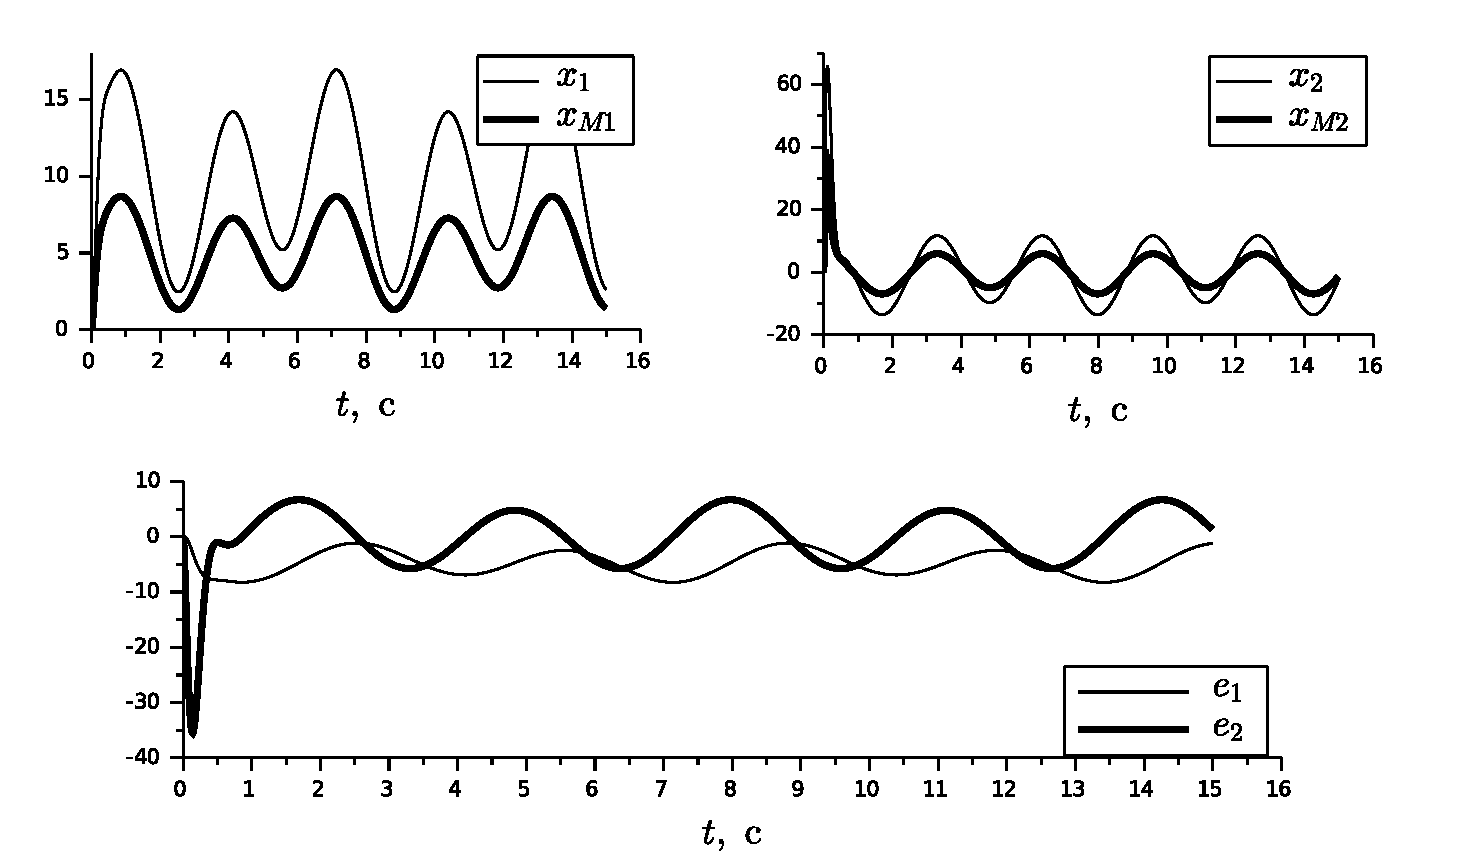
\includegraphics[width=\textwidth]{no_adapt_stable.pdf}
    \caption{Графики переходных процессов при $a_0=-125$, $a_1 = -15$ ($\theta_1 = -381$, $\theta_2 = -47$).}
\end{figure}

\vspace{1cm}

\begin{figure}[h!]
    \centering
    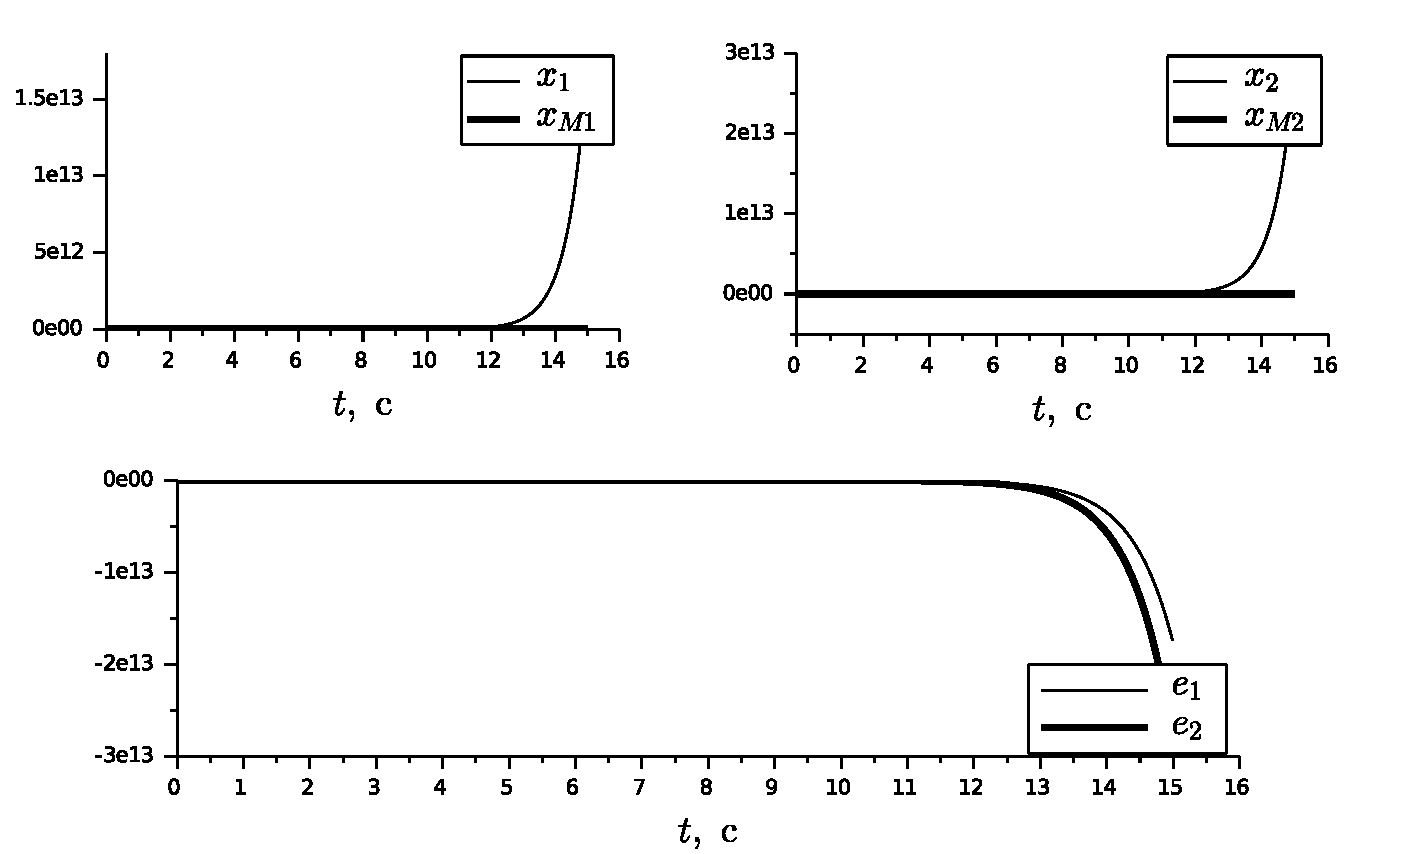
\includegraphics[width=\textwidth]{no_adapt_unstable.pdf}
    \caption{Графики переходных процессов при $a_0=-258$, $a_1 = -32$ ($\theta_1 = -514$, $\theta_2 = -64$).}
    \label{img_no_adapt_unstable}
\end{figure}


\subsection{Моделирование работы адаптивной системы}
Результаты моделирования работы адаптивной системы управления и соответствующая схема моделирования показаны на рисунках~\ref{img_adapt}--\ref{img_adapt_g_1}.

Матрица $P$, которая использовалась в экспериментах, равна:
\begin{equation}
    P = \arg \{ A_M^T P + P A_M = -I\} =
    \begin{bmatrix}4.078125&0.0019531\cr 0.0019531&0.0156860\cr \end{bmatrix}
\end{equation}

Экспериментам, чьи результаты изображены на рисунках~\ref{img_adapt_nominal}--\ref{img_adapt_unstable}, соответствует значение коэффициента адаптации, равное~$\gamma=1000$.

\vspace{1.5cm}

\begin{figure}[h!]
    \centering
    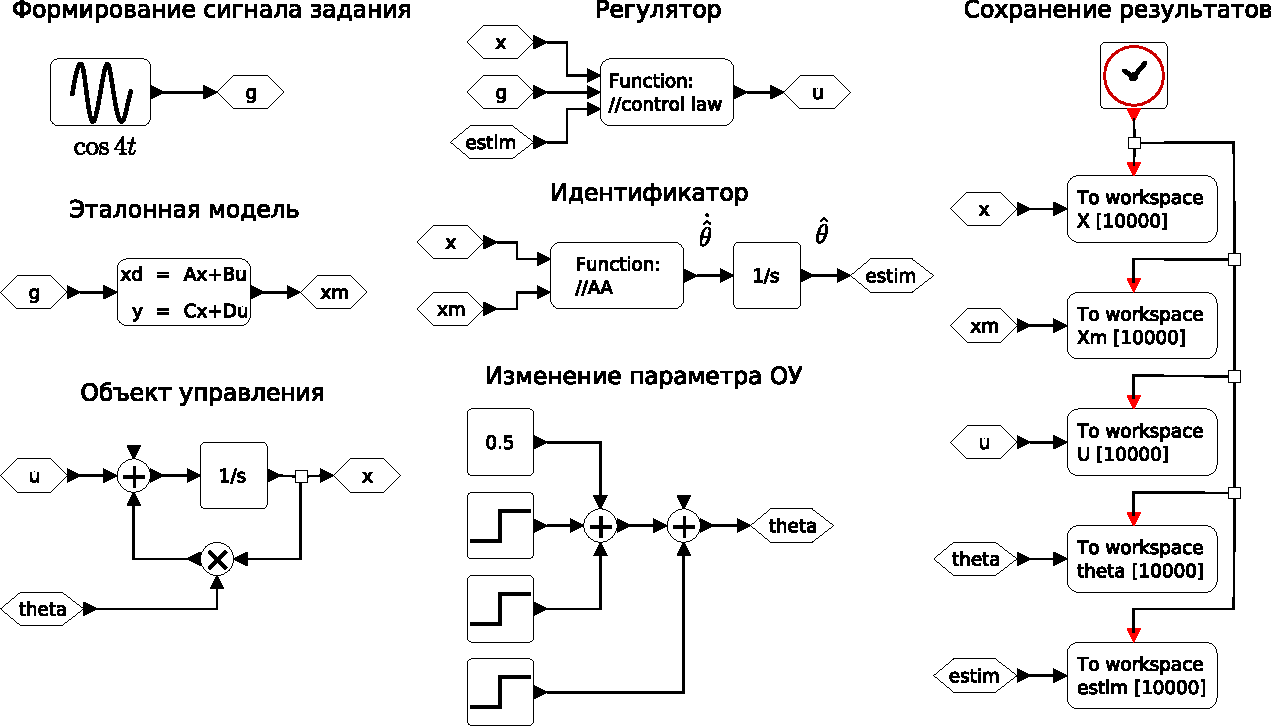
\includegraphics[width=\textwidth]{adapt.pdf}
    \caption{Схема моделирования процесса управления с помощью настраиваемого регулятора.}
    \label{img_adapt}
\end{figure}


\begin{figure}[h!]
    \centering
    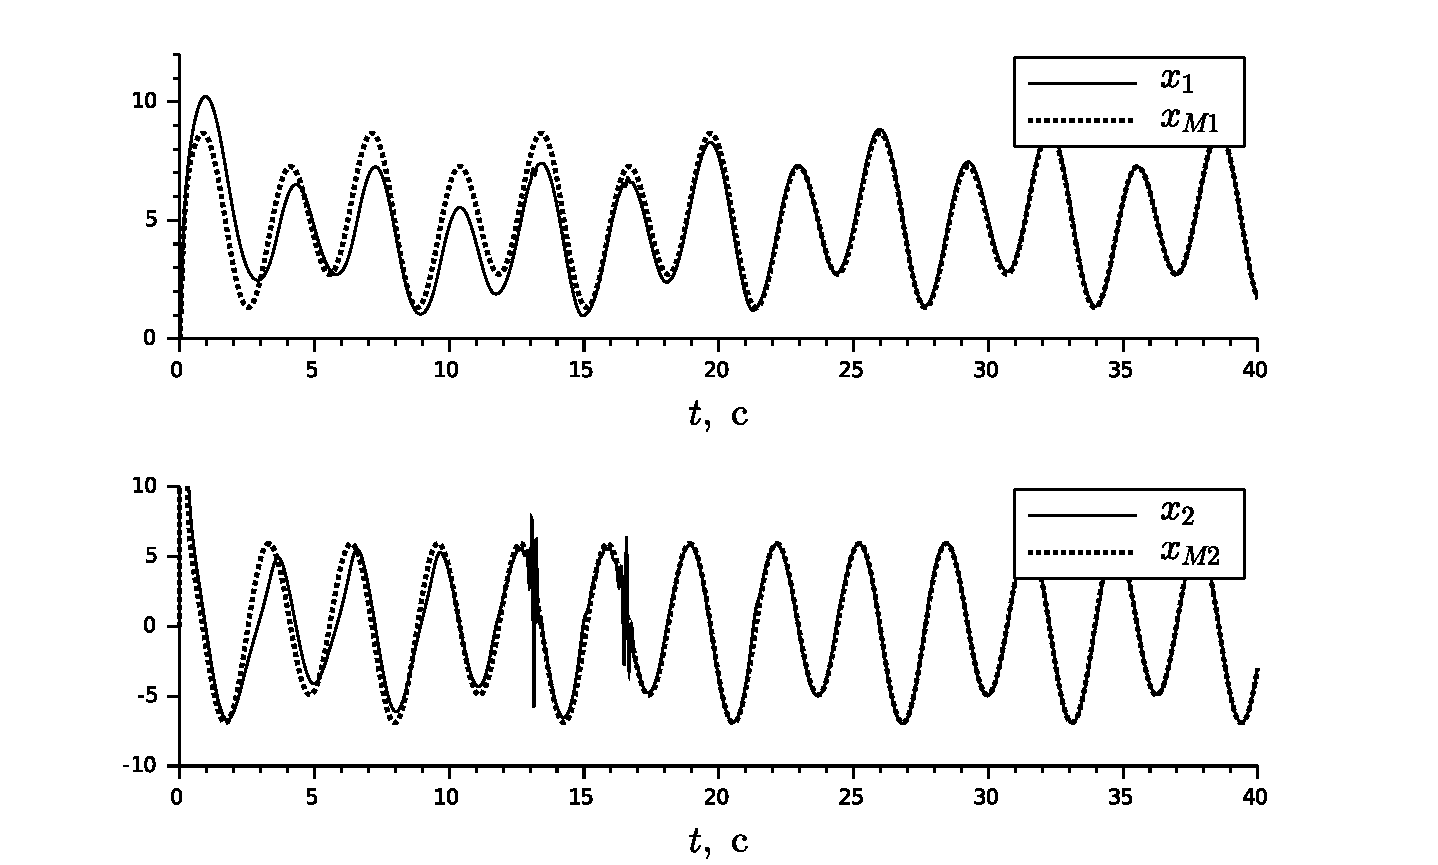
\includegraphics[width=1.05\textwidth]{adapt_nominal_1.pdf}
    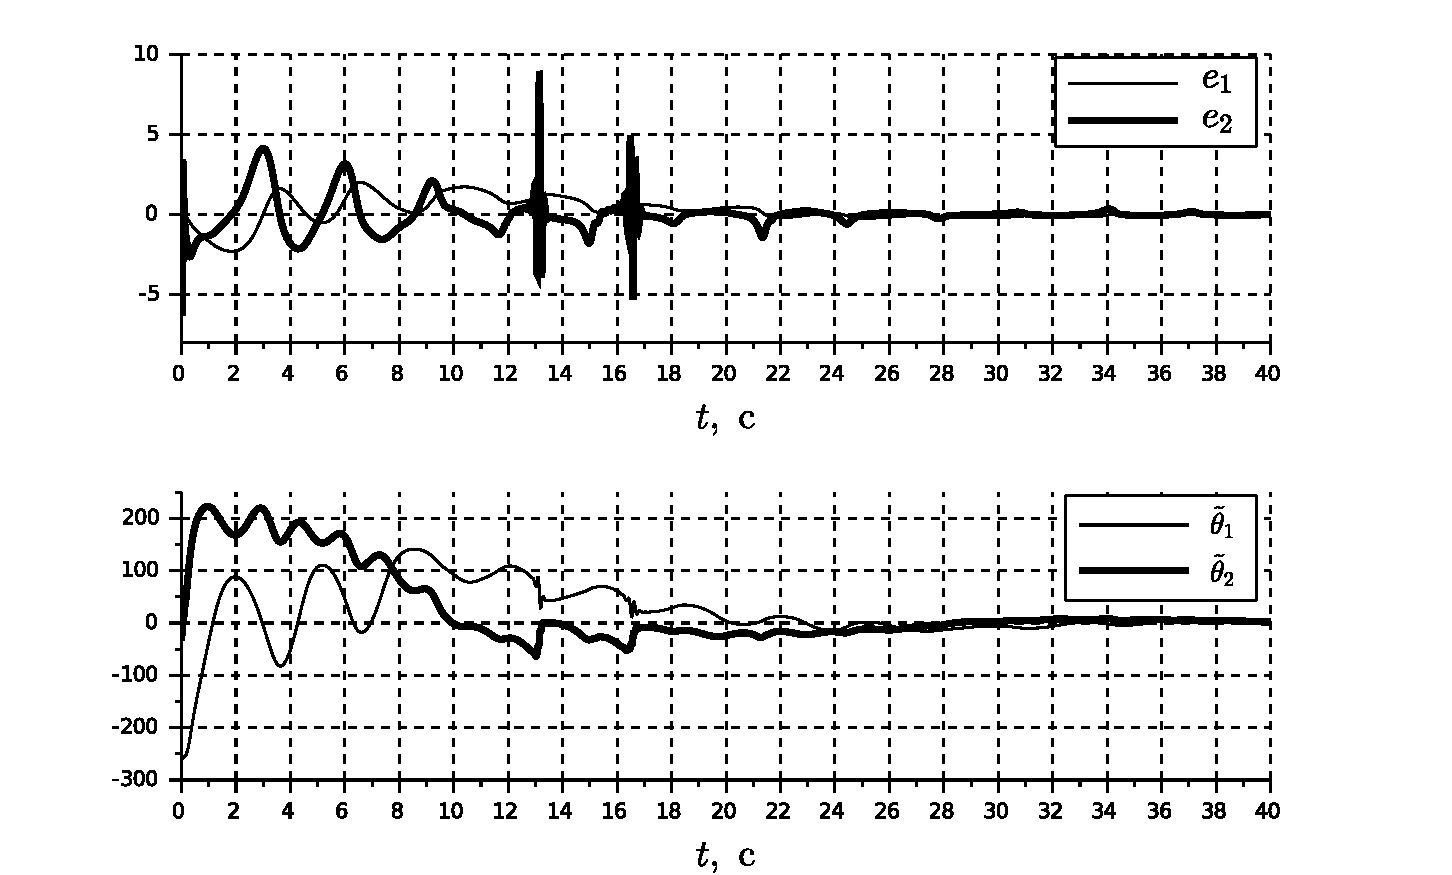
\includegraphics[width=1.05\textwidth]{adapt_nominal_2.pdf}
    \caption{Графики переходных процессов при $a_0=-1$, $a_1 = 1$ ($\theta_1 = -257$, $\theta_2 = -31$).}
    \label{img_adapt_nominal}
\end{figure}

\begin{figure}[h!]
    \centering
    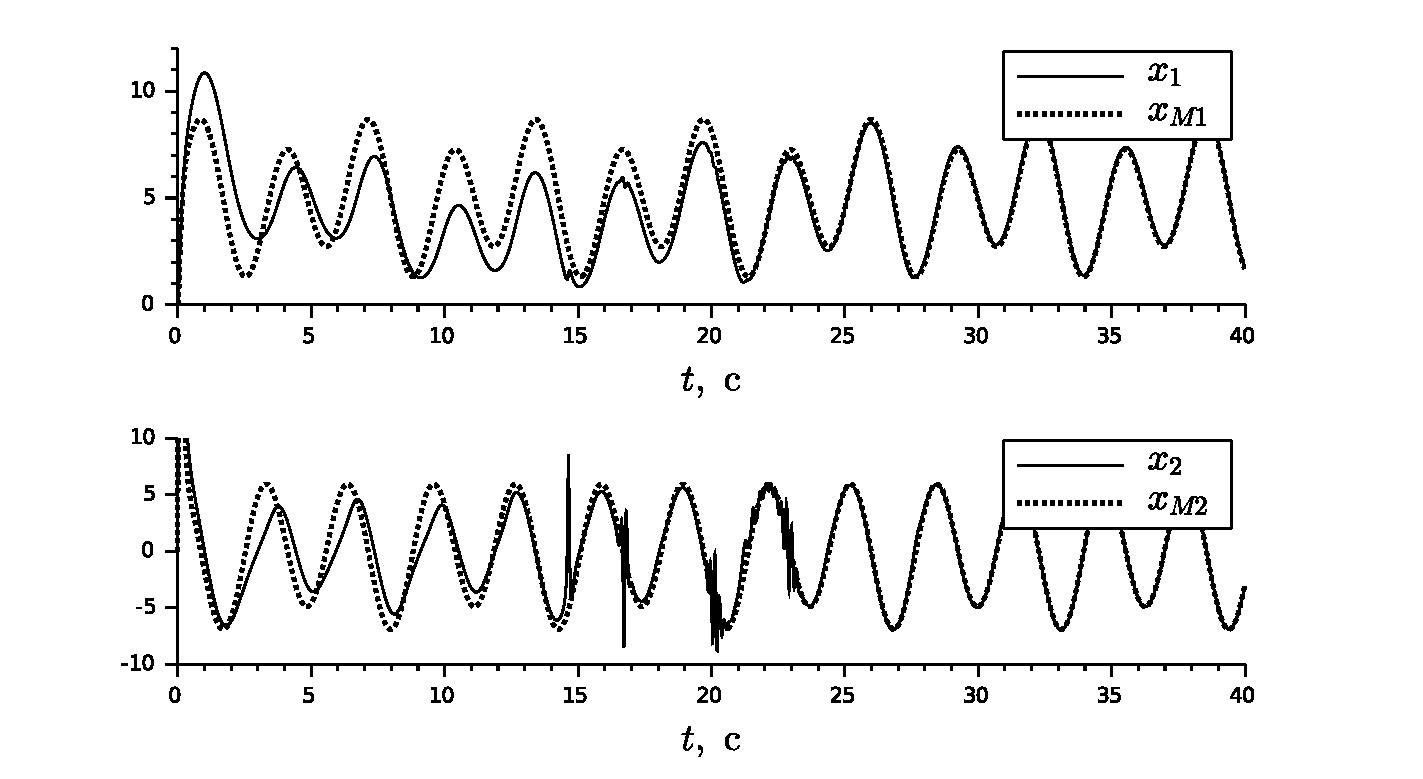
\includegraphics[width=1.05\textwidth]{adapt_stable_1.pdf}
    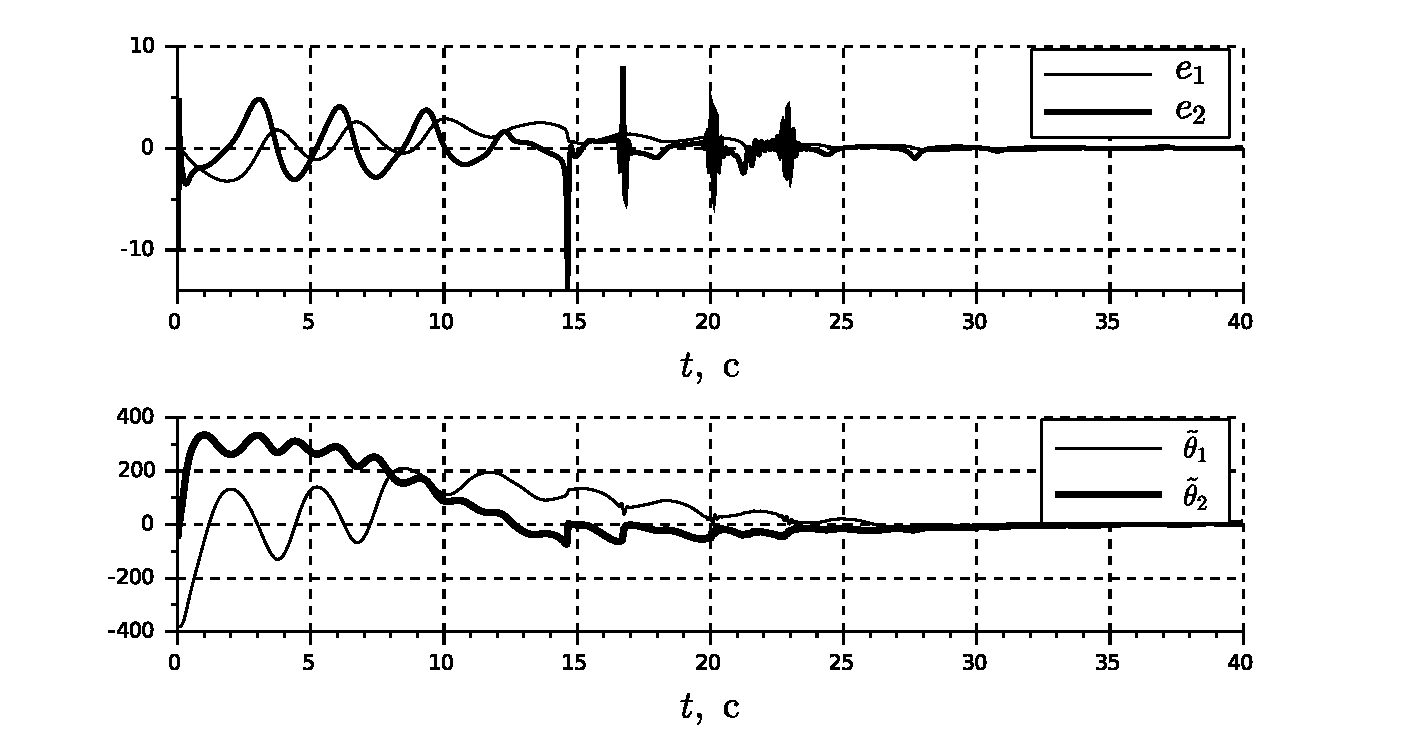
\includegraphics[width=1.05\textwidth]{adapt_stable_2.pdf}
    \caption{Графики переходных процессов при $a_0=-125$, $a_1 = -15$ ($\theta_1 = -381$, $\theta_2 = -47$).}
\end{figure}

\begin{figure}[h!]
    \centering
    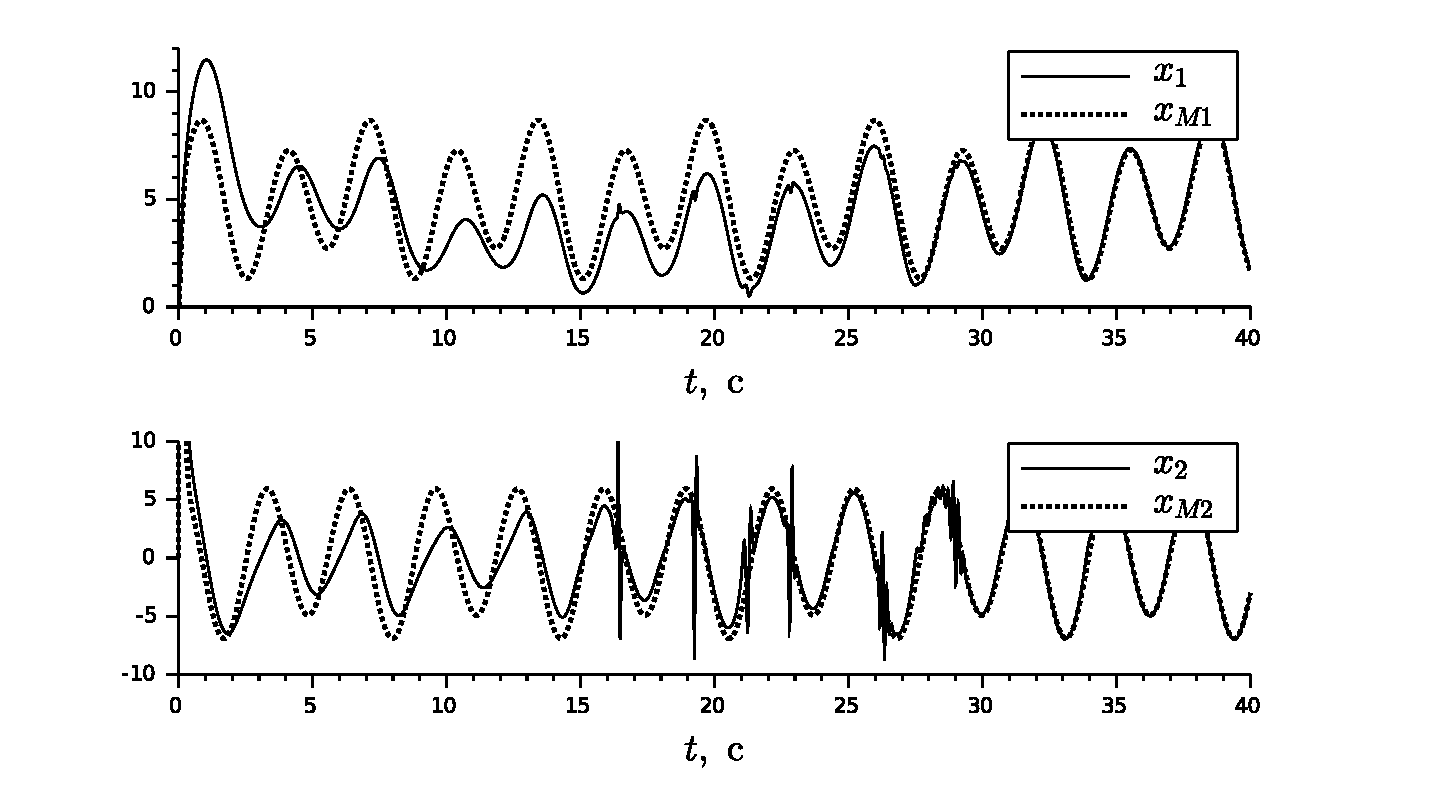
\includegraphics[width=1.05\textwidth]{adapt_unstable_1.pdf}
    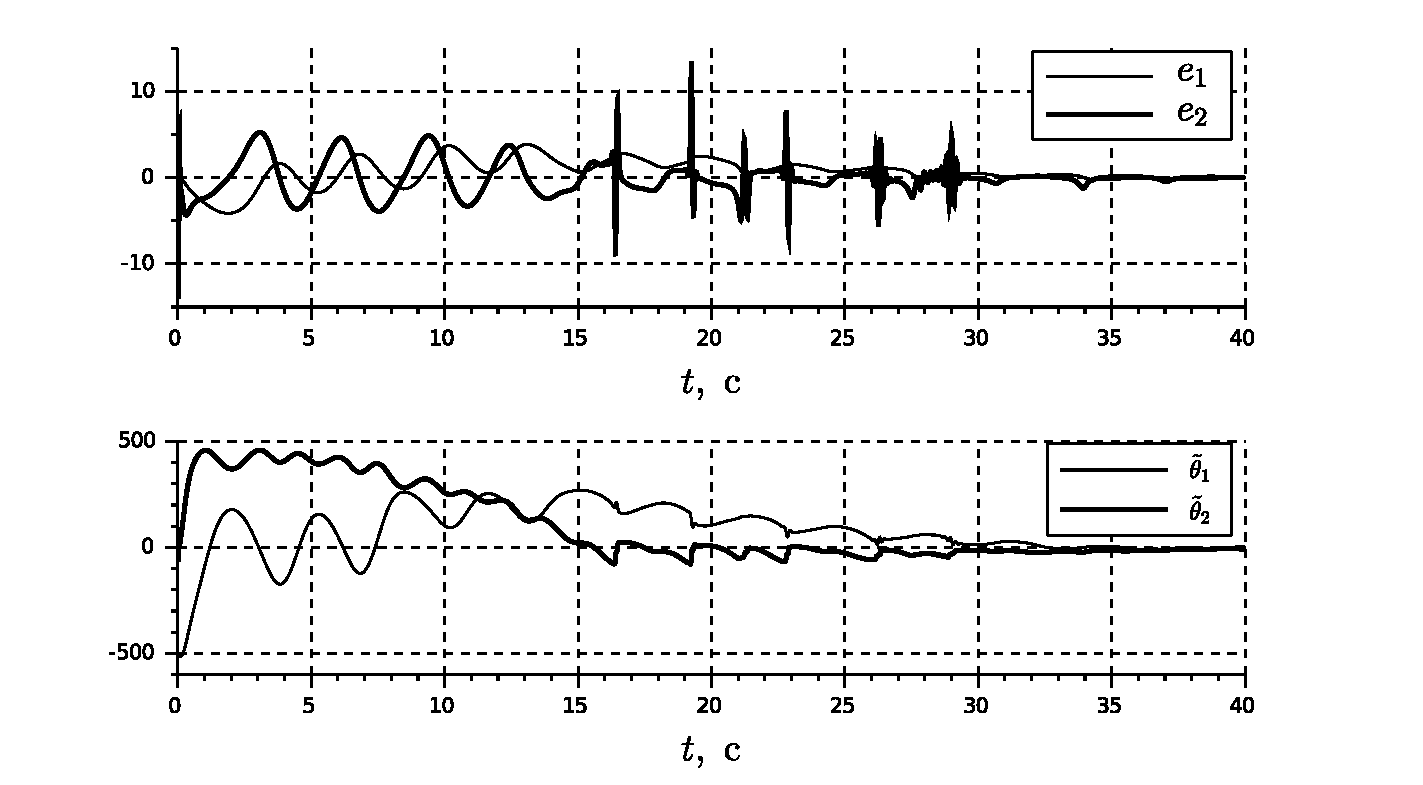
\includegraphics[width=1.05\textwidth]{adapt_unstable_2.pdf}
    \caption{Графики переходных процессов при $a_0=-258$, $a_1 = -32$ ($\theta_1 = -514$, $\theta_2 = -64$).}
    \label{img_adapt_unstable}
\end{figure}

\begin{figure}[h!]
    \centering
    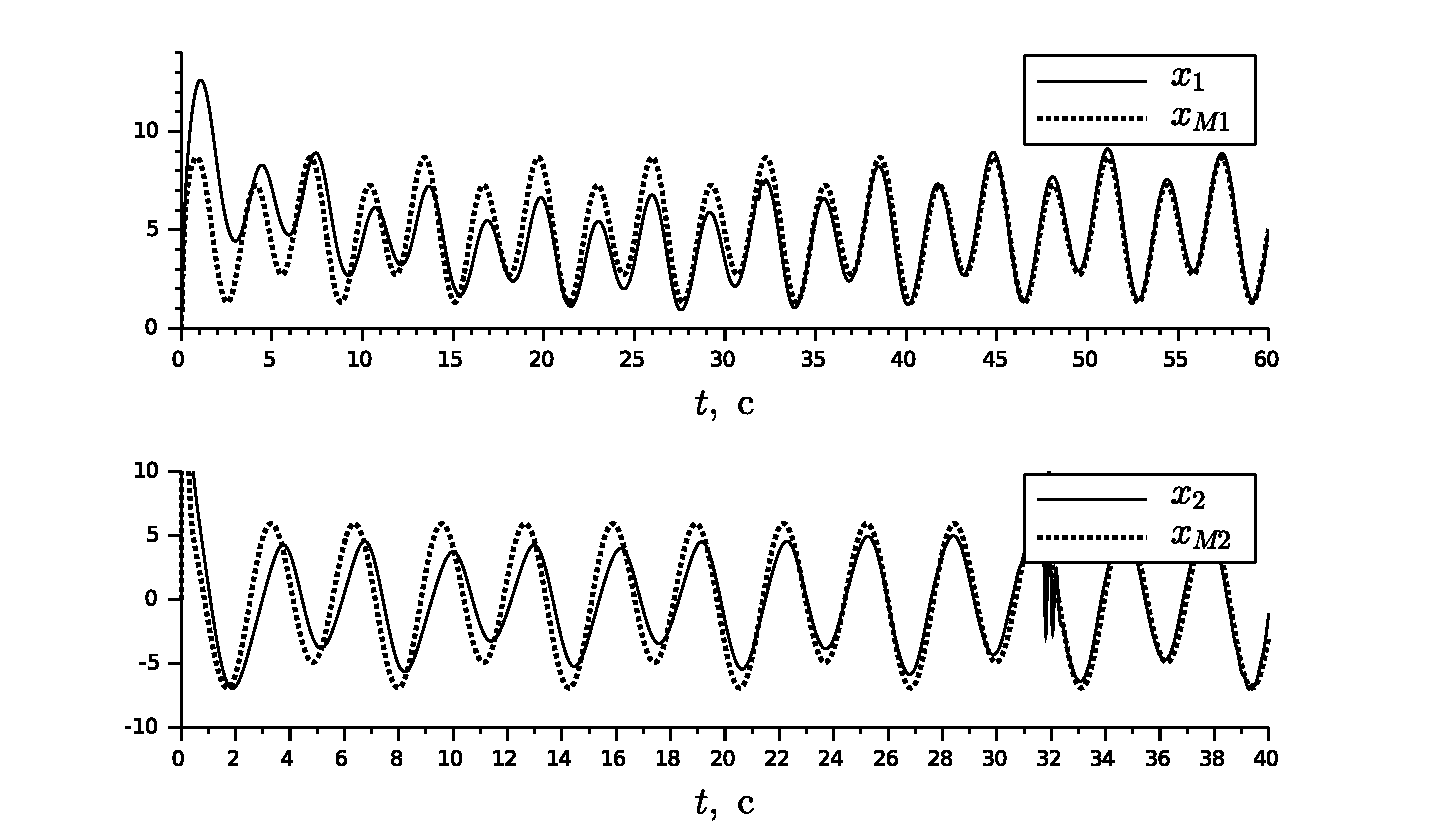
\includegraphics[width=1.05\textwidth]{adapt_gamma_250.pdf}
    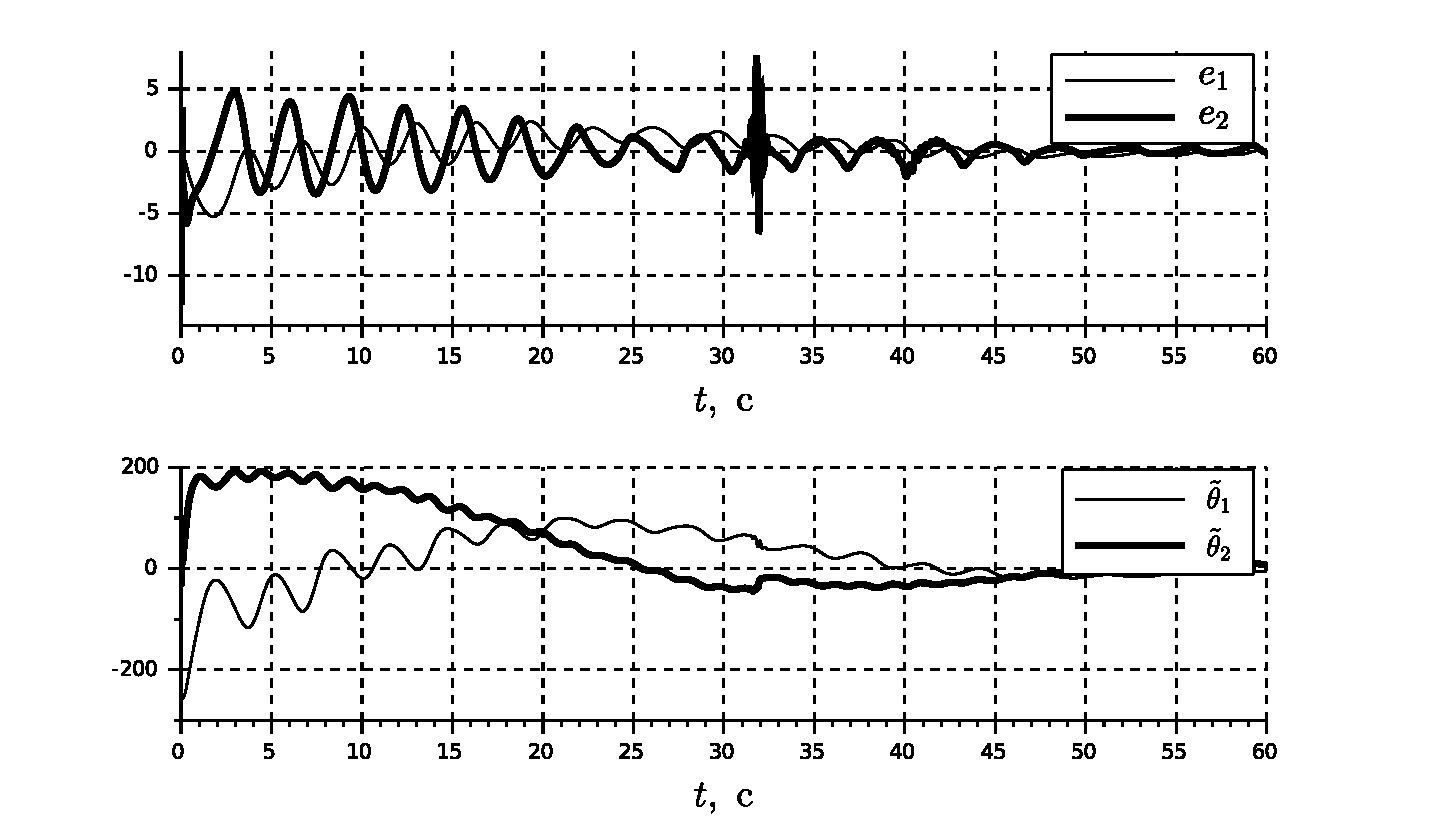
\includegraphics[width=1.05\textwidth]{adapt_gamma_250_2.pdf}
    \caption{Графики переходных процессов при $a_0=-1$, $a_1 = 1$, $\gamma = 250$.}
    \label{img_adapt_gamma_250}
\end{figure}

\begin{figure}[h!]
    \centering
    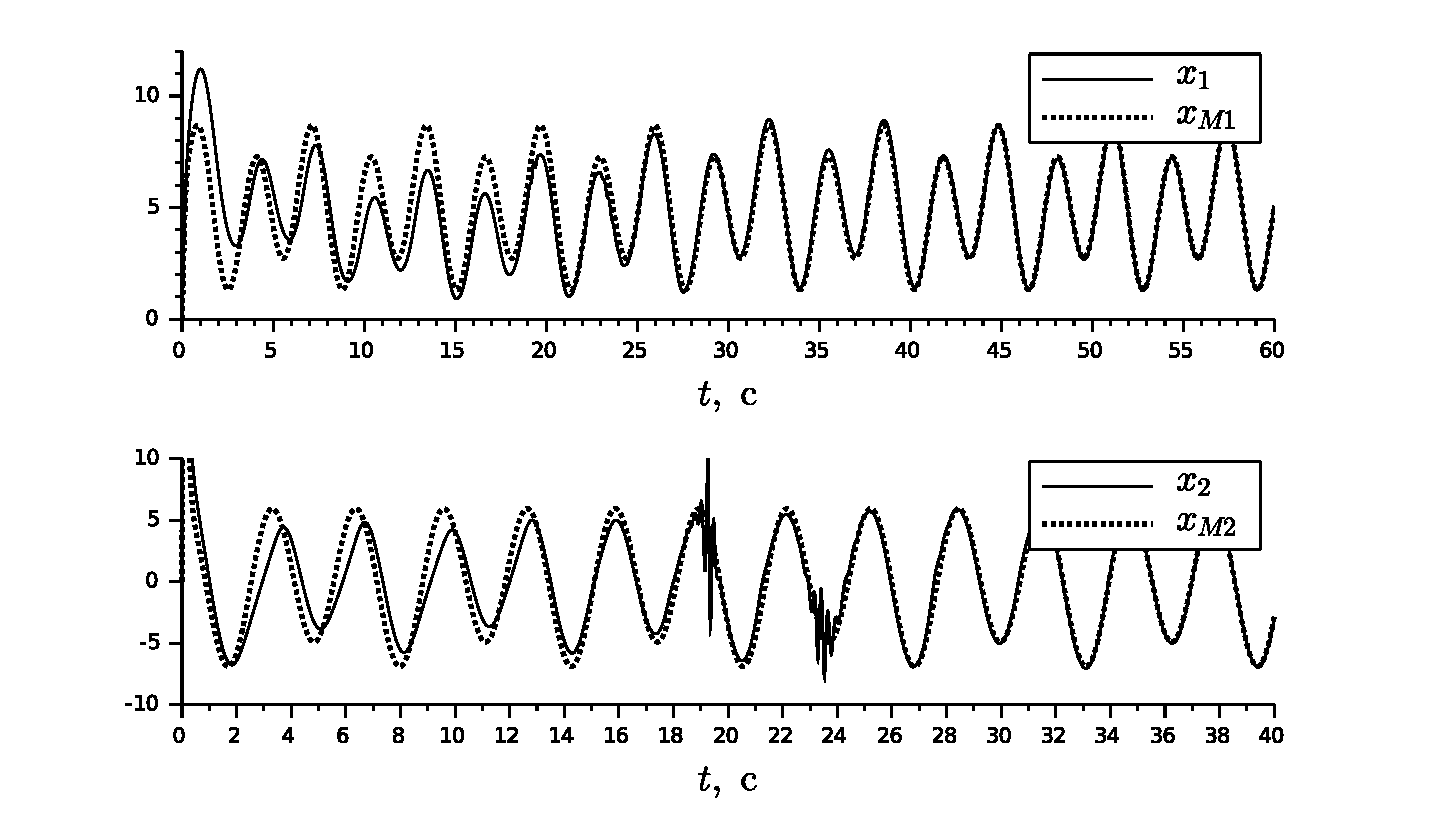
\includegraphics[width=1.05\textwidth]{adapt_gamma_500.pdf}
    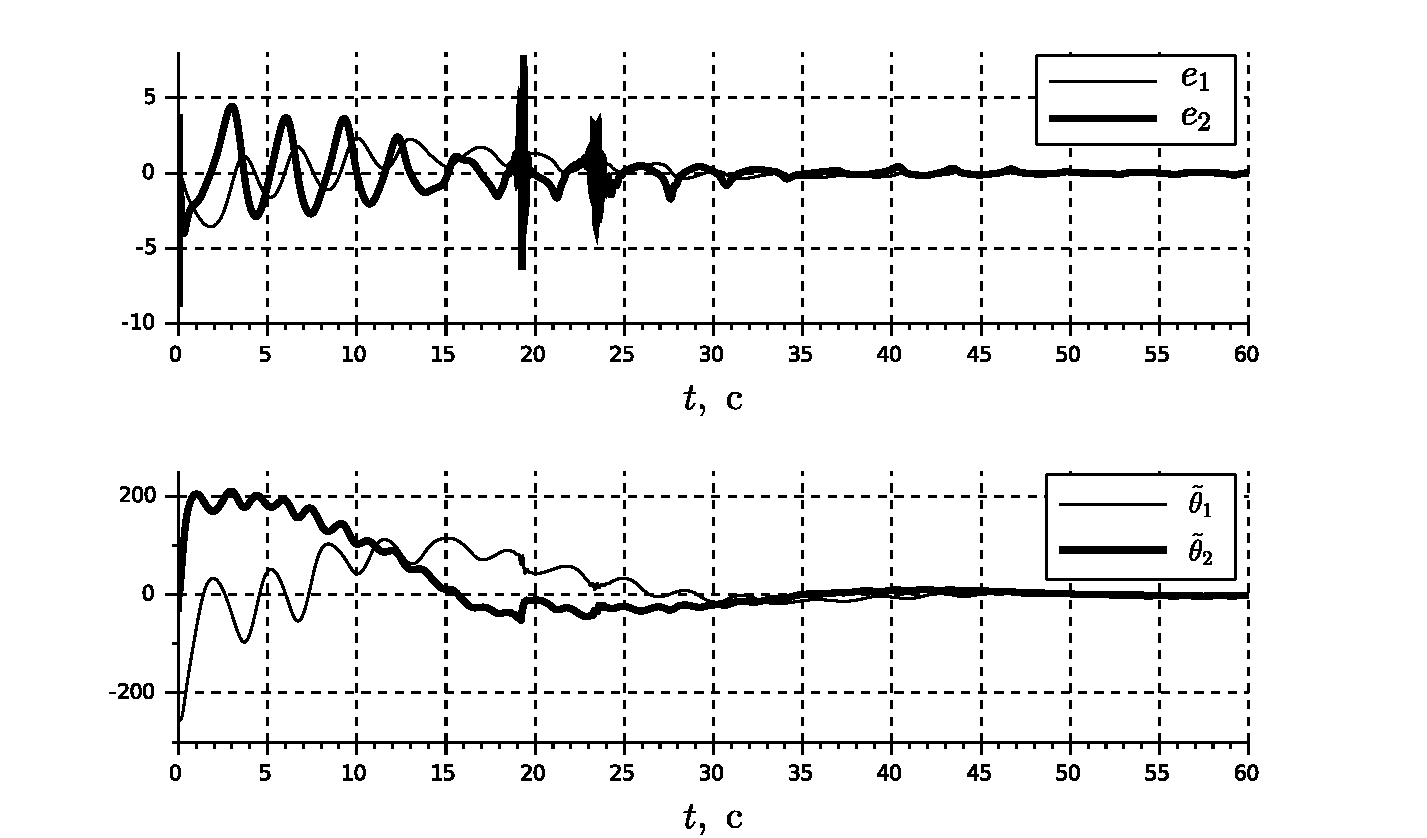
\includegraphics[width=1.05\textwidth]{adapt_gamma_500_2.pdf}
    \caption{Графики переходных процессов при $a_0=-1$, $a_1 = 1$, $\gamma=500$.}
\end{figure}

\begin{figure}[h!]
    \centering
    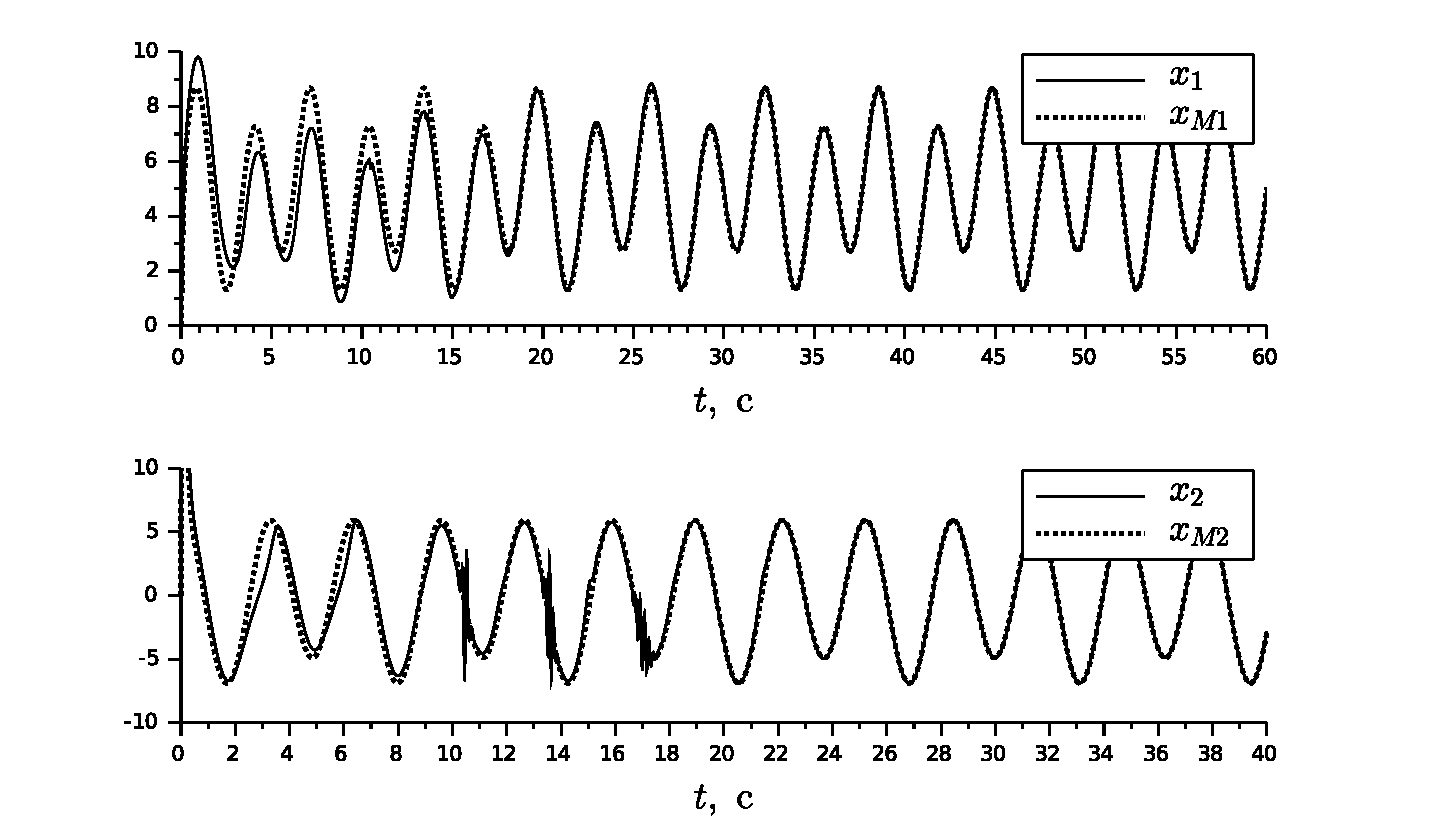
\includegraphics[width=1.05\textwidth]{adapt_gamma_1500.pdf}
    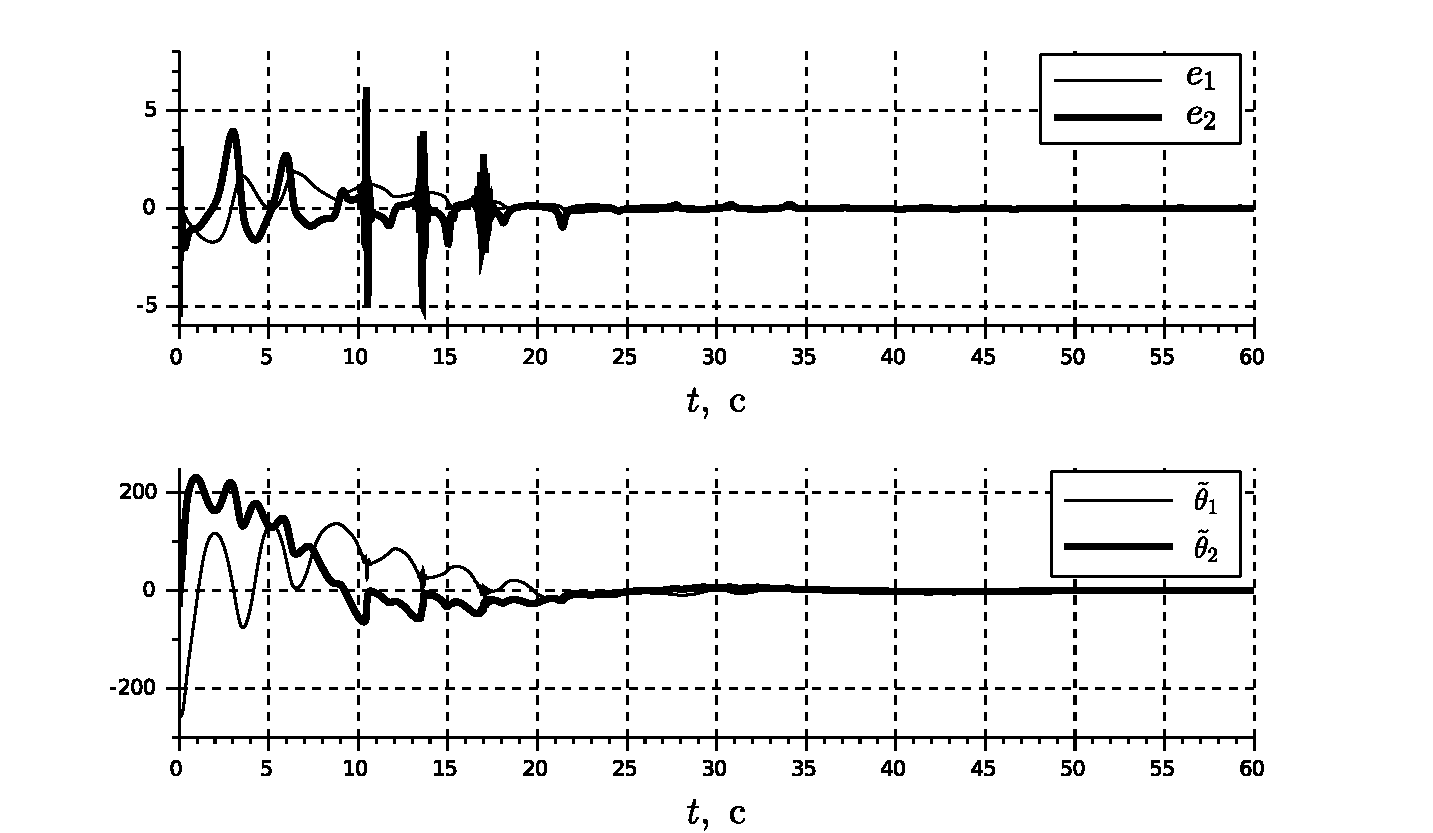
\includegraphics[width=1.05\textwidth]{adapt_gamma_1500_2.pdf}
    \caption{Графики переходных процессов при $a_0=-1$, $a_1 = 1$, $\gamma = 1500$.}
    \label{img_adapt_gamma_1500}
\end{figure}

\begin{figure}[h!]
    \centering
    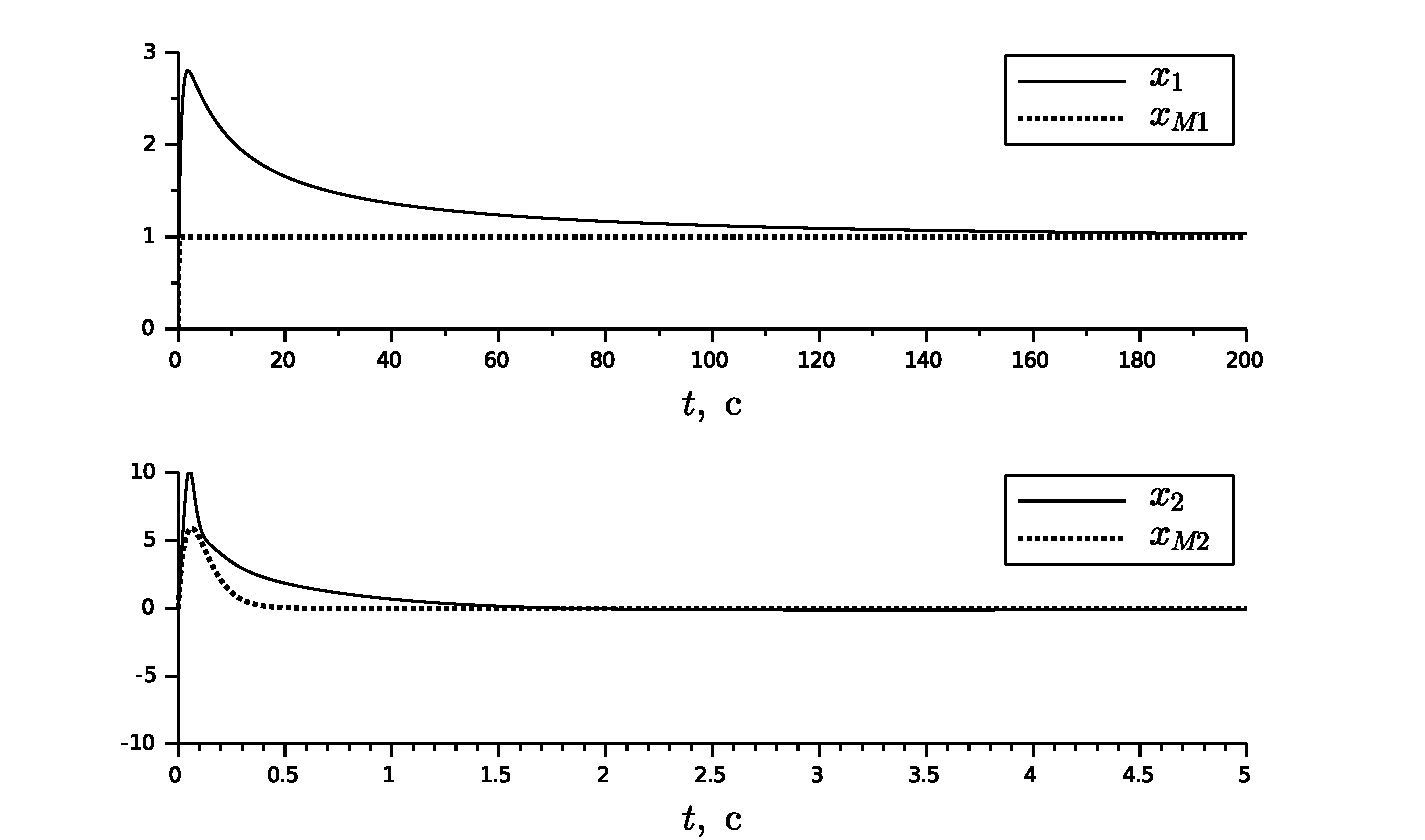
\includegraphics[width=1.05\textwidth]{adapt_g_1.pdf}
    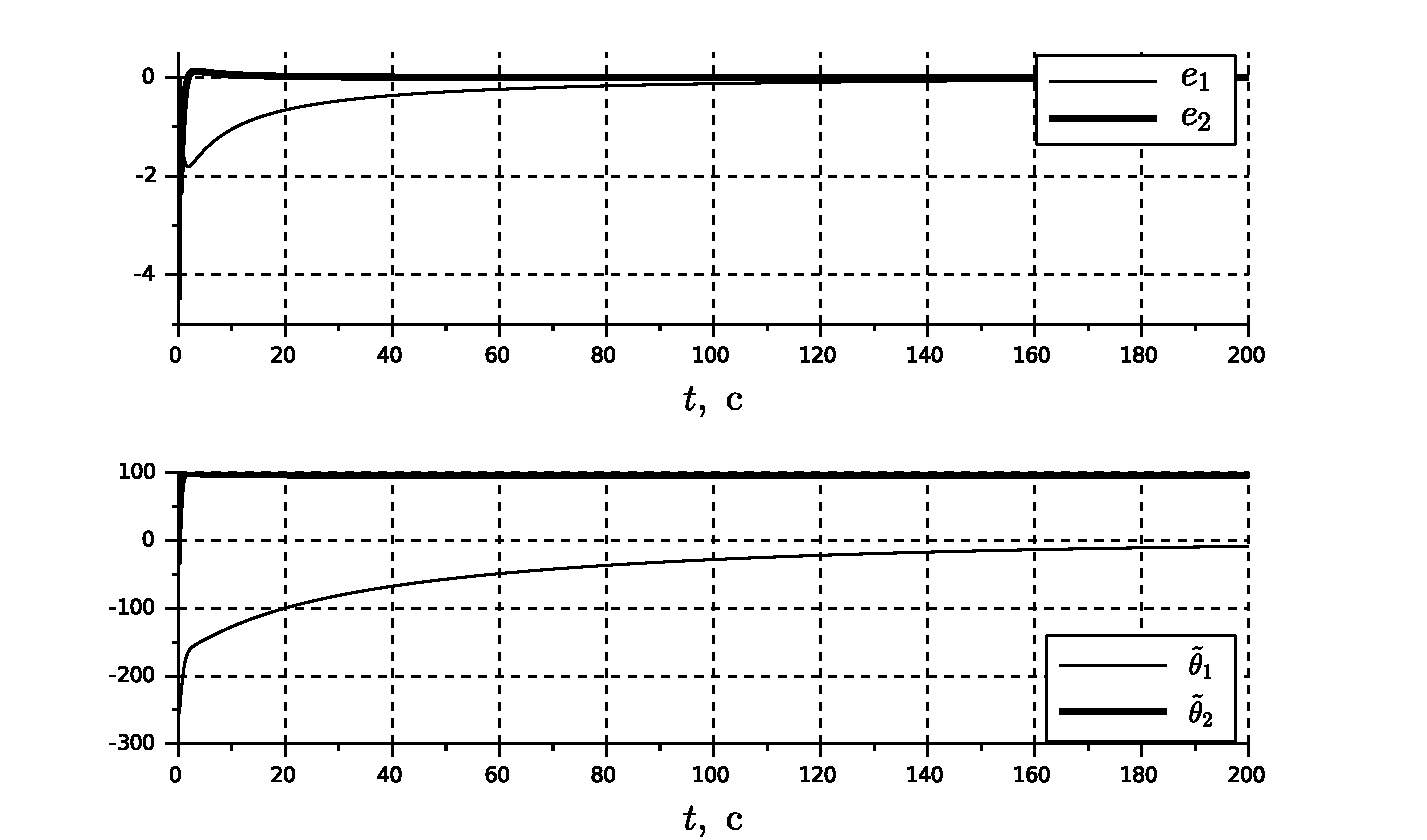
\includegraphics[width=1.05\textwidth]{adapt_g_1_2.pdf}
    \caption{Графики переходных процессов при $a_0=-1$, $a_1 = 1$ ($\theta_1 = -257$, $\theta_2 = -31$), $\gamma = 1500$ и $g(t) = 1$.}
    \label{img_adapt_g_1}
\end{figure}

\newpage
\mbox{}
\newpage
\mbox{}
\newpage
\mbox{}
\newpage
\mbox{}
\newpage
\mbox{}
\newpage
\mbox{}
\newpage
\mbox{}
\newpage
\section{Выводы по работе}
В~результате проделанной работы
\begin{itemize}
    \item была построена эталонная система, график переходной функции которой удовлетворяет заданным в работе показателям качества ($t_\text{п} = 0.3 \text{ с}, \sigma = 0\%$)~--- см. рисунок~\ref{img_ref_model};
    \item было установлено, что 
    \begin{enumerate}
        \item ненастраиваемый регулятор, получающийся из~\eqref{eq_tuned_controller} заменой $\hat{\theta}$ на $\theta$, обеспечивает целевое равенство~\eqref{eq_goal_of_control} только в том случае, если параметры объекта управления совпадают с заложенными в закон управления значениями; в противном случае регулятор не только не обеспечивает выполнение соотношения~\eqref{eq_goal_of_control}, но и может не гарантировать устойчивость итоговой системы (см.~рисунки~\ref{img_no_adapt_nominal}--\ref{img_no_adapt_unstable});
        \item применение адаптивного закона управления дает управляемому объекту способность достигать цели~\eqref{eq_goal_of_control}, а следовательно и обеспечивает его устойчивость (см.~рисунки~\ref{img_adapt_nominal}--\ref{img_adapt_unstable});
        \item значение коэффициента адаптации влияет на скорость сходимости вектора оценок~$\hat{\theta}$ к истинному значению (см.~рисунки~\ref{img_adapt_nominal} и~\ref{img_adapt_gamma_250}--\ref{img_adapt_gamma_1500});
        \item при сигнале задания $g(t)=1$ резко снижается скорость движения вектора оценок~$\hat{\theta}$ к некоторому установившемуся значению, а последнее к тому же оказывается не совпадающим с истинным значением вектора параметра~$\theta$ (см. рисунок~\ref{img_adapt_g_1}).
    \end{enumerate}
\end{itemize}